\section{Definition}
We will quickly go over some fundamental definitions.\todo{More!!!}

\subsection{Basics}
\begin{definition}[Multilayer Perceptron]\label{def:mlp}
    Multilayer perceptrons are a class of functions from $\Rb^n$ to $\Rb^m$, with $n,m \in \Nb$. In this thesis, we define a multilayer perceptron as a finite sequence, such that a multilayer perceptron $\mlp$ is defined as $\mlp := (\mlp)_{i\in[k]}$ where $k$ is the number of layers. For every $i \in [k]$, the $i$.th layer of the $\mlp$ is the $i$.th item in the finite sequence $(\mlp)_i$. Further, all layers are recursively defined as:
    \begin{align*}
        (\mlp)_{1}(v) &:= v\\
        (\mlp)_{i+1}(v) &:= \sigma(W_i \cdot (\mlp)_{i} (v) + b_i), \quad \forall i \in [k-1]
    \end{align*}
    where $\sigma$ is an element wise activation function, $W_i$ is the weight matrix and $b_i$ the bias vector of layer $i$. Note, that for each $W_i$, the succeeding $W_{i+1}$ must have the same number of columns as $W_i$ has rows, in order to be well-defined. Similarly, for every layer $i$, $W_i$ and $b_i$ have to have the same number of rows.
    Following this definition, when applying a $\mlp$ on input $v \in \Rb^n$ it is $\mlp(v) := (\mlp)_k(v)$.
\end{definition}

\subsubsection{Permutation-invariance and -equivariance}
We use $S_n$ to denote the symmetric group over the elements $[n]$ for any $n > 0$. $S_n$ consists of all permutations over these elements. Let $G$ be a graph with $V(G) = [n]$, applying a permutation $\pi \in S_n$ on $G$, is defined as $G_\pi := \pi \cdot G$ where $V(G_\pi) = \{\pi(1), \ldots, \pi(n) \}$ and $E(G_\pi) = \{ (\pi(v), \pi(u)) \mid (v,u) \in E(G)\}$. We will now introduce two key concepts for classifying functions on graphs.

\begin{definition}[Permutation Invariant]
    Let $f: \mathcal{G} \rightarrow \mathcal{X}$ be an arbitrary function and let $V(G) = [n]$ for some $n \in \mathbb{N}$. The function $f$ is \textit{permutation-invariant} if and only if for all $G \in \mathcal{G}$ where $n_G := \mid V(G) \mid$ and for every $\pi \in S_{n_G}$: $f(G) = f(\pi \cdot G)$.
\end{definition}

\begin{definition}[Permuation Equivariant]
    Let $f: \mathcal{G} \rightarrow \mathcal{X}$ be an arbitrary function and let $V(G) = [n]$ for some $n \in \mathbb{N}$. The function $f$ is \textit{permuation-equivariant} if and only if for all $G \in \mathcal{G}$ where $n_G := \mid V(G) \mid$ and for every $\pi \in S_{n_G}$: $f(G) = \pi^{-1} \cdot f(\pi \cdot G)$.
\end{definition}

\subsection{Weisfeiler and Leman Algorithm}\label{sec:1-WL Definition}
The Weisfeiler-Leman algorithm consists of two main parts, first the coloring algorithm and second the graph isomorphism test. We will introduce them in this section.

\subsubsection{The Weisfeiler-Leman graph coloring algorithm}

\begin{definition}[$\wl$ Algorithm]
Let $G = (V, E, l)$ be a graph, then in each iteration $i$, the 1-WL computes a node coloring $C_i: V(G) \rightarrow \mathbb{N}$, which depends on the coloring of the neighbors and the node itself. In iteration $i=0$, the initial coloring is $C_0 = l$ or if $l$ is non-existing $C_0(v) = c$ for all $v \in V(G)$ for an arbitrary constant $c \in \mathbb{N}$. For $i > 0$, the algorithm assigns a color to $v \in V(G)$ as follows:
\begin{equation*}
C_i (v) = \textsf{RELABEL}(C_{i-1}(v), \MSopen C_{i-1}(u) \mid u \in \mathcal{N}(v) \MSclose),
\end{equation*}

\noindent where $\textsf{RELABEL}$ injectively maps the above pair to a unique, previously not used, natural number. Although this is not a formal restriction by the inventors, we further require the function to always map to the next minimal natural number. Thereby we can contain the size of the codomain of each coloring for all iterations. The algorithm terminates when the number of colors between two iterations does not change, meaning the algorithm terminates after iteration $i$ if the following condition is satisfied:
\begin{equation*}
\forall v,w \in V(G):  C_i(v) = C_i(w) \iff C_{i+1}(v) = C_{i+1}(w).
\end{equation*}
Upon terminating we define $C_{\infty}$:= $C_i$ as the stable coloring, such that $\wl(G) := C_\infty$. The algorithm always terminates after $n_G:= |V(G)|$ iterations (\cite{Gro2017}). 
\end{definition}
For an illustration of this coloring algorithm, see \autoref{Encoding example}. Moreover, based on the work of \cite{Pai+87} about efficient refinement strategies, \cite{Car+82} proved that the stable coloring $C_\infty$ can be computed in time $\mathcal{O}(| V(G) | + |E(G)| \cdot \log | V(G) |)$.\todo{Bring many infos outside of the definiton. And add that we call this algorihm $\wl$.}

\subsubsection{The Weisfeiler-Leman Graph Isomorphism Test}

\begin{definition}[$\wl$ Isomorphism Test]
    To determine if two graphs $G, H \in \mathcal{G}$ are non-isomorphic ($G \ncong H)$, one applies the 1-WL coloring algorithm on both graphs ``in parallel'' and checks after each iteration if the occurrences of each color are equal, else the algorithm would terminate and conclude non-isomorphic. Formally, the algorithm concludes non-isomorphic in iteration $i$ if there exists a color $c$ such that: 
    \begin{equation*}
        |\{ v \in V(G) \mid c = C_i(v)\} | \neq |\{ v \in V(H) \mid c = C_i(v)\} |.
    \end{equation*}
\end{definition}
Note that this test is only sound and not complete for the \textit{graph isomorphism problem}. Counterexamples where the algorithm fails to distinguish non-isomorphic graphs can be easily constructed, see \autoref{1-WL Counter Example} which was discovered and proven by \cite{Cai1992}.
\begin{figure}[H]
    \centering
    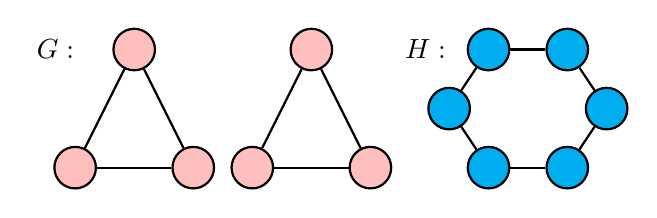
\begin{tikzpicture}

\tikzset{line/.style={draw,thick}}
\tikzset{arrow/.style={line,->,>=stealth}}
\tikzset{node/.style={circle,inner sep=0pt,minimum width=15pt}}

\draw (-1.0,0.75) node {$G:$};
\node[line,node,fill=pink] (x1) at (0, 0.75) {};
\node[line,node,fill=pink] (x2) at (-0.75, -0.75) {};
\node[line,node,fill=pink] (x3) at (0.75, -0.75) {};

\path[line] (x1) to (x2);
\path[line] (x1) to (x3);
\path[line] (x2) to (x3);

\node[line,node,fill=pink] (x1) at (2.25, 0.75) {};
\node[line,node,fill=pink] (x2) at (1.5, -0.75) {};
\node[line,node,fill=pink] (x3) at (3.0, -0.75) {};

\path[line] (x1) to (x2);
\path[line] (x1) to (x3);
\path[line] (x2) to (x3);

\draw (3.7, 0.75) node {$H:$};
\node[line,node,fill=cyan] (x1) at (3.75 + 0.25, 0) {};
\node[line,node,fill=cyan] (x2) at (4.25 + 0.25, 0.75) {};
\node[line,node,fill=cyan] (x3) at (5.25 + 0.25, 0.75) {};
\node[line,node,fill=cyan] (x4) at (5.75 + 0.25, 0) {};
\node[line,node,fill=cyan] (x5) at (5.25 + 0.25, -0.75) {};
\node[line,node,fill=cyan] (x6) at (4.25 + 0.25, -0.75) {};

\path[line] (x1) to (x2);
\path[line] (x2) to (x3);
\path[line] (x3) to (x4);
\path[line] (x4) to (x5);
\path[line] (x5) to (x6);
\path[line] (x6) to (x1);

\end{tikzpicture}
    \caption{An example of two graphs $G$ and $H$ that are non-isomorphic but cannot be distinguished by the 1-WL.}
    \label{1-WL Counter Example}
\end{figure}

\subsection{$\wlnn$}
Text ABC \todo{Here to do}

\begin{definition}[$\wlnn$]
    We say the function $\cB: \mathcal{G} \rightarrow \Rb^m$ is computable by $\wlnn$, if it can be compromised as $\cB(\cdot) = \text{MLP} \circ f_{\text{enc}} \circ \wl(\cdot)$, where $f_{\text{enc}}$ is an encoding function that maps graph coloring to fixed-sized vectors, and $\mlp$ is a multilayer perceptron. \todo{f must be permutation invariant?}
\end{definition}

As a concrete example of a collection of functions computable by $\wlnn$ we will introduce the collection $\mathfrak{B}_k$ that is parametrized by $k \in \Nb_{\geq 1}$. All functions $\cB \in \mathfrak{B}_k$ use the \emph{counting-encoding} function $f_{\text{count}}$ as their encoding function, and are constrained in their domain to only work over a subset $\cX$ of $\cG$. We will define this particular encoding function in the following:
\begin{definition}[Counting Encoding Functions]
    For $k \in \mathbb{N}$, let 
    \begin{equation*}
        \mathcal{X} = \{ G \in \mathcal{G} \mid \forall x \in V(G) \cup E(G): l_G(x) \leq k \} \subset \cG
    \end{equation*}
        be the set of all graphs, where the label alphabet $\Sigma$ of the respective label function $l$ is bounded with $\Sigma \subseteq [k]$. We define the \emph{counting-encoding} function $f_{\text{count}}: \mathcal{X} \rightarrow \mathbb{N}^K$ as the function that maps a graph coloring $C_\infty$ of a graph $G \in \cX$ to a vector $v \in \mathbb{N}^K$ such that the $c$.th component of $v$ is equal to the number of occurrences of the color $c$ in the coloring $C_\infty$. More formally, for $G \in \mathcal{X}$ let $C_\infty$ be the final coloring upon the termination of the 1-WL algorithm on $G$ and $h_{G, C_\infty}$ the respective color histogram. Then $F$ maps $G$ to a vector $v \in \mathbb{N}^K$, such that for all $c \in [K]: v_c = h_{G, C_\infty}(c)$, where $v_c$ denotes the $c$.th component of the vector $v$. Important to note, due to the bounded label alphabet $\Sigma$ of all graphs $G 
    \in \mathcal{X}$ by the parameter $k$, there exists a minimal $K$ for the codomain $\Nb^K$ of $f_{\text{count}}$, such that $f_{\text{count}}$ is well-defined on all graphs $G \in \mathcal{X}$.
\end{definition}

To illustrate how this encoding function works and why we coined it \emph{counting-encoding}, we will quickly introduce an example graph $G$. In \autoref{Encoding example}, we give a visual representation of $G$ and its stable coloring after applying the 1-WL algorithm to it. The \emph{counting-encoding} function $f_{\text{count}}$ counts through all colors $i \in [K]$ and sets each $i$.th component of the output vector to the number of occurrences in the final coloring. Therefore, the respective color histogram $h_{G, C_\infty} = \MSopen 2, 2, 3, 4 \MSclose$ of $G$ is being mapped to $v \in \mathbb{N}^K$ with $v = (0, 2, 1, 1,0,  \dots ,0)^T$, since color $2$ appears two times, while color $3$ and $4$ occur only once. All other components of $v$ are set to $0$.
\begin{figure}[H]
    \centering
    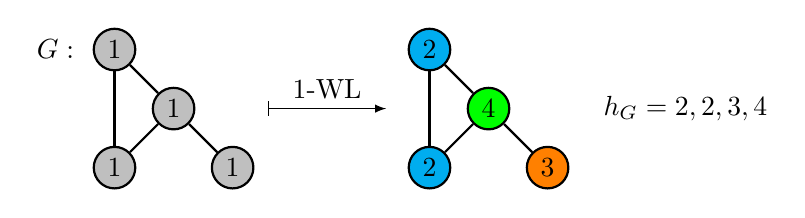
\begin{tikzpicture}
    \tikzset{line/.style={draw,thick}}
    \tikzset{arrow/.style={line,->,>=stealth}}
    \tikzset{node/.style={circle,inner sep=0pt,minimum width=15pt}}
    
    \draw (-1.5,0.75) node {$G:$};
    \node[line,node,fill=lightgray] (x1) at (-0.75, 0.75) {1};
    \node[line,node,fill=lightgray] (x2) at (-0.75, -0.75) {1};
    \node[line,node,fill=lightgray] (x3) at (0.75, -0.75) {1};
    \node[line,node,fill=lightgray] (x4) at (0, 0) {1};
    
    \path[line] (x1) to (x2);
    \path[line] (x1) to (x4);
    \path[line] (x2) to (x4);
    \path[line] (x3) to (x4);

    \draw [|-latex] (1.2,0) -- node [text width=2.5cm,midway,above,align=center ] {1-WL} (2.7,0);
    

    \node[line,node,fill=cyan] (x1) at (-0.75 + 4.0, 0.75) {2};
    \node[line,node,fill=cyan] (x2) at (-0.75 + 4.0, -0.75) {2};
    \node[line,node,fill=orange] (x3) at (0.75 + 4.0, -0.75) {3};
    \node[line,node,fill=green] (x4) at (0 + 4.0, 0) {4};
    
    \path[line] (x1) to (x2);
    \path[line] (x1) to (x4);
    \path[line] (x2) to (x4);
    \path[line] (x3) to (x4);

    \draw (6.5, 0.0) node {$h_G = \MSopen 2, 2, 3, 4 \MSclose$};

    
    
    \end{tikzpicture}

    \caption{An example of the final coloring computed by applying the 1-WL algorithm on the graph $G$. The graph $G$ consists of $4$ nodes with all their labels being initially set to $1$. Note that each label corresponds to a color, which we have also plotted for illustration purposes.}
    \label{Encoding example}
\end{figure}

\subsection{Graph Neural Networks (Message Passing)}\label{sec:GNN Defintion}
Let $G = (V, E, l)$ be an arbitrary graph. A Graph Neural Network (GNN) is a composition of multiple layers where each layer $t$ passes a vector representation of each node $v$ or edge $e$ through $f^{(t)}(v)$ or $f^{(t)}(e)$ respectively and retrieves thereby a new graph that is structurally identical but has new feature information. Note that in the following we will restrict the definition to only consider node features, however, one can easily extend it to also include edge features.\todo{Better intro text}

\begin{definition}[Graph Neural Network]
    Let $G = (V, E, l)$ be an arbitrary graph. A Graph Neural Network (GNN) is a composition of multiple layers where each layer $t$ is represented by a function $f^{(t)}$ that works over the set of nodes $V(G)$. To begin with, we need a function $f^{(0)}: V(G) \rightarrow \mathbb{R}^{1 \times d}$ that is consistent with $l$, that translates all labels into a vector representation. Further, for every $t > 0$, $f^{(t)}$ is of the format:
    \begin{align*}
    f^{(t)}(v) = f^{W_{1,t}}_{\text{merge}} (f^{(t-1)}(v), \  f^{W_{2,t}}_{\text{agg}}( \MSopen f^{(t-1)}(w) \mid w \in \mathcal{N}(v) \MSclose )),
    \end{align*}
    where $f^{W_{1,t}}_{\text{merge}}$ and $f^{W_{2,t}}_{\text{agg}}$ are arbitrary differentiable functions with $W_{1,t}$ and $W_{2,t}$ their respective parameters. Additionally, $f^{W_{2,t}}_{\text{agg}}$ has to be permuation-invariant.

    Depending on the objective, whether the GNN is tasked with a graph or a node task, the last layer differs. In the case of graph tasks, we add a permutation-invariant aggregation function to the end, here called $\textsf{READOUT}$, that aggregates over every node and computes a fixed-size output vector for the entire graph, e.g. a label for graph classification. In order to ensure that we can train the GNN in an end-to-end fashion, we require $\textsf{READOUT}$ to be also differentiable. Let $\mathcal{A}$ be an instance of the described GNN framework. Further, let $K \in \mathbb{N}$ be the number of layers of the GNN, $\mathcal{G}$ the set of all graphs, $\mathcal{Y}$ the task-specific output set (e.g. labels of a classification task), then the overall function computed by $\mathcal{A}$ is:
    \begin{align*}
        &\mathcal{A}: \mathcal{G} \rightarrow \mathcal{Y}: x \mapsto \textsf{READOUT} \circ f^{(K)} \circ \ldots \circ f^{(0)}(x),
    \end{align*}
    if $\mathcal{A}$ is configured for a graph task, otherwise:
    \begin{align*}
        &\mathcal{A}: \mathcal{G} \rightarrow \mathcal{Y}: x \mapsto f^{(K)} \circ \ldots \circ f^{(0)}(x).
    \end{align*}
\end{definition}

Note that, as we require all aggregation functions to be permutation-invariant, the total composition $\mathcal{A}$ is permutation-invariant, and with similar reasoning, it is also differentiable. This enables us to train $\mathcal{A}$ like any other machine learning method in an end-to-end fashion, regardless of the underlying encoding used for graphs. This definition and use of notation are inspired by \cite{Morris2018} and \cite{Xu2018}.

To demonstrate what kind of functions are typically used, we provide functions used by \cite{Ham+2017} for a node classification:
\begin{align*}
f^{W_{1,t}}_{\text{merge}}(v) &= \sigma (W_{\text{merge}} \cdot \textsf{concat}(f^{(t-1)}(v), \ f^{W_{2,t}}_{\text{agg}}(v)))\\
f^{W_{2,t}}_{\text{agg}}(v) &= \max(\{ \sigma(W_{\text{pool}} \cdot f^{(t-1)}(u) + b) \mid u \in \mathcal{N}(v)\})
\end{align*}
where $\sigma$ is a non-linear element wise activation function; $W_{\text{merge}}$, $W_{\text{pool}}$ are trainable matrices, $b$ a trainable vector and \textsf{concat} the concatenation function.



\subsection{Important for later}
\begin{definition}[1-WL Relation]
    For any graphs $G,H$ we will denote $G \wliso H$ if the 1-WL isomorphism test can not distinguish both graphs. Note that due to the soundness of this algorithm, if $G \not\wliso H$, we always can conclude that $G \not\simeq H$.
\end{definition}

\begin{definition}[$\wldisc$]
    Let $\mathcal{C}$ be a collection of permutation invariant functions from $\mathcal{X}^{n\times n}$ to $\Rb$. We say $\mathcal{C}$ is \textbf{\wldisc} if for all graphs $G_1, G_2 \in \mathcal{X}$ for which the 1-WL isomorphism test concludes non-isomorphic ($G_1 \not\wliso G_2$), there exists a function $h \in \mathcal{C}$ such that $f(G_1) \neq f(G_2)$.
\end{definition}

\begin{definition}[$\gapp$]
    Let $\mathcal{C}$ be a collection of permutation invariant functions from $\mathcal{X}^{n\times n}$ to $\Rb$. We say $\mathcal{C}$ is \textbf{\gapp} if for all permutation-invariant functions $\mathcal{A}$ computed by a GNN, and for all $\epsilon \in \Rb$ with $\epsilon > 0$, there exists $h_{\cA,\epsilon} \in \mathcal{C}$ such that $\| \cA - h_{\cA,\epsilon} \|_\infty := \sup_{G \in \mathcal{X}} |f(G) - h_{\cA,\epsilon}(G)| < \epsilon$
\end{definition}

\section{Theorems}
Throughout this thesis we will concentrate on a finite collection of finite graphs which we will denote with $\cX \subset \cG$.

\begin{theorem}[Finite Case: ``$\wlnn \subseteq \text{GNN}$'']\label{theorem:1wl_in_gnn}
    Let $\cC$ be a collection of functions from $\cX$ to $\Rb$ computable by GNNs, then $\cC$ is also computable by $\wlnn$.
\end{theorem}

\begin{theorem}[Finite Case: ``$\text{GNN} \subseteq \wlnn$'']
    Let $\cC$ be a collection of functions from $\cX$ to $\Rb$ computable by $\wlnn$, then $\cC$ is also computable by GNNs.
\end{theorem}


\subsection{Proof of \cref{theorem:1wl_in_gnn}}
We will prove \cref{theorem:1wl_in_gnn} by introducing a couple of small lemmas, which combined prove the theorem. In detail, in \cref{lem:wl_disc_exists} we show the existence of a collection computed by $\wlnn$ that is 1-\!WL-Discriminating. In \cref{lem:wlnn_permutation_invariance,lem:wl_relation_equivalence,lem:composition_lemma} we derive properties of $\wlnn$ functions we will use throughout \cref{lem:encoding-indicator-func1,lem:encoding-indicator-func2,lem:decompose_gnn_as_wl} with which we prove the theorem.
We took great inspiration for \cref{lem:encoding-indicator-func1,lem:encoding-indicator-func2,lem:decompose_gnn_as_wl} from the proof presented in section 3.1 in the work of \cite{Chen2019}.

\begin{lemma}\label{lem:wl_disc_exists}
    There exists a collection $\cC$ of functions from $\cX$ to $\Rb$ computable by $\wlnn$ that is 1-\!WL-Discriminating.
\end{lemma}
\begin{proof}
We consider the collection $\mathfrak{B}_k$ of functions from $\cX$ to $\Rb$ computed by \wlnn, where we choose $k$ as follows:
\begin{equation*}
    k := \max \bigl( \{ l_G(v) \mid G \in \cX, v \in V(G)\} \bigr),
\end{equation*}
the largest label of any node of any graph in $\cX$. Note that we can compute $k$, since $\cX$ is finite.

Let $G_1, G_2 \in \cX$ such that the 1-WL isomorphism test concludes non-isomorphic ($G_1 \not\wliso G_2$). We denote with $(C_{\infty})_G$ the final coloring computed by the 1-WL algorithm when applied on $G$.
Due to $G_1 \not\wliso G_2$, there exists a color $c \in \Nb$ such that $h_{G_1, (C_\infty)_{G_1}}(c) \neq h_{G_2, (C_\infty)_{G_1}}(c)$. If we now consider as mu the following function $\text{MLP}_c: \Nb^K \rightarrow \Rb, v \mapsto W \cdot v$ with $W \in \Nb^{1 \times K}$ such that $W_{1,c} := 1$ and $W_{1,i} := 0$ for all $i \in [K] \setminus \{c\}$, we can construct $\cB$ as $\cB(\cdot) := \mlp \circ f_{\text{count}} \circ \wl(\cdot)$. Then $\cB(G) := h_{G, (C_\infty)_G}(c)$, such that we can conclude $\mathcal{B}(G_1) \neq \mathcal{B}(G_2)$, 


Then we can conclude that $\mathcal{B}(G_1) \neq \mathcal{B}(G_2)$. Since $G_1,G_2$ are arbitrary, we can conclude the proof.
\end{proof}

\begin{lemma}[$\wlnn$ Equivalence]\label{lem:wl_relation_equivalence}
    Let $\cC$ be a collection of functions computable by $\wlnn$, then for every function $\cB \in \cC$ and every pair of graphs $G_1, G_2 \in \xnn:$ if $G_1 \wliso G_2$ than $\cB(G_1) = \cB(G_2)$.
\end{lemma}

\begin{proof}
    Let $\cC$ be a collection of functions computed by $\wlnn$. Let $\cB$ be an arbitrary function in $\cC$, then $\cB$ is comprised as follows: $\cB(\cdot) = \text{MLP} \circ f_{\text{enc}} \circ \wl(\cdot)$. Let $G_1, G_2 \in \xnn$ be arbitrary graphs with $G_1 \wliso G_2$, then by definition of the relation $\wliso$ we know that $\wl(G_1) = \wl(G_2)$. With this the equivalence follows immediatly.
\end{proof}

\begin{lemma}[$\wlnn$ Permuation Invariance]\label{lem:wlnn_permutation_invariance}
    Let $\cC$ be a collection of functions computable by $\wlnn$, then every function $\cB \in \cC$ is permutation-invariant.
\end{lemma}

\begin{proof}
    Let $\cC$ be a collection of functions computable by $\wlnn$. Let $G_1, G_2 \in \xnn$ be arbitrary graphs with $G_1 \simeq G_2$ and $\cB$ be an arbitrary function in $\cC$. Since the $\wl$ algorithm is sound, we know that $G_1 \simeq G_2$ implies $G_1 \wliso G_2$. Using \cref{lem:wl_relation_equivalence}, we can therefore conclude that: $\cB(G_1) = \cB(G_2)$.
\end{proof}

\begin{lemma}[$\wlnn$ Composition]\label[lemma]{lem:composition_lemma}
    Let $\cC$ be a collection of functions computable by $\wlnn$. Further, let $h_1, \dots h_n \in \cC$ and $\mlp^\bullet$ an multilayer perceptron, than the function $\cA$ composed of $\cA(\cdot) := \text{MLP}(h_1(\cdot), \ldots, h_n(\cdot))$ is also computable by $\wlnn$.
\end{lemma}
\begin{proof}
    Assume the above and let $f_{1}, \ldots, f_{n}$ be the encoding functions, as well as $\text{MLP}_1, \ldots, \text{MLP}_n$ be the multilayer perceptrons used by $h_1, \dots h_n$ respectively. The idea of this proof is, we construct an encoding function $f^*$ that maps a coloring $C_\infty$ to a concatenation of the vectors obtained when applying each encoding function $f_i$ individually. Additionally, we construct a multilayer perceptron $\mlp^*$ that takes in this concatenation of vectors and simulates all $\text{MLP}_1, \ldots, \text{MLP}_n$ simultaneously on their respective section of the encoding vector of $f^*$, and applies afterwards the given $\mlp^\bullet$ on the concatenation of the output of all $\mlp_i$'s.  See \autoref{fig:proof_idea_parallelism} for a sketch of the proof idea. A complete proof can be found in the Appendix, as this proof is very technical and not that interesting.

    \begin{figure}[H]
        \centering
        \begin{tikzpicture}

    \tikzset{line/.style={draw,thick}}
    \tikzset{arrow/.style={line,->,>=stealth}}
    \tikzset{node/.style={circle,inner sep=0pt,minimum width=15pt}}
    
    \node (inputG) {$G$};
    \node (coloring) [right =of inputG] {$M_G$};
    \node (firstV) [right =of coloring] {$\begin{bmatrix*}
        f_1(M_G)\\
        \vdots\\
        f_n(M_G)
    \end{bmatrix*}$};
    \node (inp1) [above right =of firstV] {$f_1(M_G)$};
    \node (inp2) [below right =of firstV] {$f_n(M_G)$};
    \node (out1) [right =of inp1] {$o_1$};
    \node (out2) [right =of inp2] {$o_n$};
    \node (out) [below right =of out1, above right =of out2] {$\begin{bmatrix*}
        o_1\\
        \vdots\\
        o_n
    \end{bmatrix*}$};
    \node (dot1) [right =of firstV] {$\vdots$};
    \node (final_out) [right =of out] {$O$};
    \node (dot2) [below =of out1] {$\vdots$};

    

    \draw[|-latex] (inputG.east) to node[text width=2.5cm,midway,above,align=center] {$\wl$} (coloring.west);

    \draw[-latex] (coloring.east) to node[text width=2.5cm,midway,above,align=center] {$f^*$} (firstV.west);

    \draw[-latex] (firstV.east) -- (inp1.west);

    \draw[-latex] (firstV.east) -- (inp2.west);

    \draw[|-latex] (inp1.east) to node[text width=2.5cm,midway,above,align=center] {$\text{MLP}_1$} (out1.west);

    \draw[|-latex] (inp2.east) to node[text width=2.5cm,midway,above,align=center] {$\text{MLP}_n$} (out2.west);

    \draw[-latex] (out1.east) -- (out.west);
    \draw[-latex] (out2.east) -- (out.west);

    \draw[|-latex] (out.east) to node[text width=2.5cm,midway,above,align=center] {$\mlp^\bullet$} (final_out.west);

    %\draw [thick, decoration={brace,mirror,raise=0.5cm},decorate, below =of out2] (firstV.south) -- (final_out.west);


    %\draw (-1.5,0.75) node {$\cA(G):$};
    %\draw (-1.0, 0.0) node {$G$};

    %\draw [|-latex] (-0.6,0) -- node [text width=2.5cm,midway,above,align=center ] {1-WL} (1.0,0);

    %\draw (1.6, 0.0) node {$(M_G)_G$};

    %\draw [|-latex] (2.4, 0.0) -- node [text width=2.5cm,midway,above,align=center ] {$f$} (3.25, 0.0);
    
    %\draw (3.5, 0.0) node {$v$};

    %\draw (5.0, 1.0) node {$v$};
    %\draw (5.0, -1.0) node {$v$};
    
\end{tikzpicture}
        \caption{Sketch of the proof we use to prove lemma XYZ.}
        \label{fig:proof_idea_parallelism}
    \end{figure}
\end{proof}
    


\begin{lemma}\label[lemma]{lem:encoding-indicator-func1}
    Let $\cC$ be a collection of functions from $\xnn$ to $\Rb$ computable by $\wlnn$ that is $\wldisc$. Then for all $G \in \xnn$, there exists a function $h_G$ from $\xnn$ to $\Rb$ computable by $\wlnn$, such that for all $G^* \in \xnn: h_G(G^*) = 0$ if and only if $G \wliso G^*$.
\end{lemma}

\begin{proof}
    For any $G_1, G_2 \in \xnn$ with $G_1 \not\wliso G_2$ let $f_{G_1, G_2} \in \cC$ be the function distinguishing them, with $f_{G_1, G_2}(G_1) \neq f_{G_1, G_2}(G_2)$. We define the function $\overline{f}_{G_1,G_2}$ working over $\xnn$ as follows:
    \begin{align}\label{eq:lem:encoding-indicator-func2}
        \overline{f}_{G_1, G_2}(\cdot) &= |f_{G_1, G_2}(\cdot) - f_{G_1, G_2}(G_1)| \nonumber \nonumber\\
        &= \max(f_{G_1, G_2}(\cdot) - f_{G_1, G_2}(G_1)) + \max(f_{G_1, G_2}(G_1) - f_{G_1, G_2}(\cdot))
    \end{align}
    Note, that in the formula above ``$f_{G_1, G_2}(G_1)$'' is a fixed constant and the resulting function $\overline{f}_{G_1, G_2}$ is non-negative.
    Let $G_1 \in \xnn$ now be fixed, we will construct the function $h_{G_1}$ with the desired properties as follows:
    \begin{align*}
        h_{G_1}(x) = \sum_{G_2 \in \xnn, \ G_1 \not\wliso G_2} \overline{f}_{G_1, G_2}(x).
    \end{align*}
    Since $\cX$ is finite, the sum is finite and therefore well-defined. Next, we will prove that for a fixed graph $G_1 \in \xnn$, the function $h_{G_1}$ is correct on input $G^* \in \xnn$:
    \begin{enumerate}
        \item If $G_1 \wliso G^*$, then for every function $\overline{f}_{G_1, G_2}$ of the sum with $G_1 \not\wliso G_2$, we know, using \cref{lem:wl_relation_equivalence}, that $\overline{f}_{G_1, G_2}(G^*)$ is equal to $\overline{f}_{G_1, G_2}(G_1)$ which is by definition $0$, such that $h_{G_1}(G^*) = 0$.
        \item If $G_1 \not\wliso G^*$, then $\overline{f}_{G_1, G^*}(G^*)$ is a summand of the overall sum, and since $\overline{f}_{G_1, G^*}(G^*) > 0$, 
        we can conclude $h_{G_1}(G*) > 0$ due to the non-negativity of each function $\overline{f}$.
    \end{enumerate}

    This function can be encoded in an MLP by replacing the $\max$ terms of the last line in \autoref{eq:lem:encoding-indicator-func2} by the activation function ReLU. Therefore, we can conclude with \cref{lem:composition_lemma} that for every graph $G$, $h_G$ is also $\wlnn$ computable.
\end{proof}

\begin{lemma}\label[lemma]{lem:encoding-indicator-func2}
    Let $\mathcal{C}$ be a collection of functions from $\mathcal{X}^{n \times n}$ to $\Rb$ computable by $\wlnn$ so that for all $G \in \mathcal{X}^{n \times n}$, there exists $h_G \in \mathcal{C}$ satisfying $h_G(G^*) = 0 $ if and only if $G \wliso G^*$ for all $G^* \in \mathcal{X}^{n \times n}$. Then for every $G \in \xnn$, there exists a function $\varphi_G $ computable by $\wlnn$ such that for all $G^* \in \xnn$: $\varphi_G(G^*) = \mathds{1}_{G \wliso G^*}$.
\end{lemma}
\begin{proof}
    Assuming the above. Due to $\cX$ being finite, we can define for every graph $G$ the constant:
    \begin{equation*}
        \delta_G := \frac{1}{2} \min_{G^* \in \xnn , G \not\wliso G^*} |h_G(G^*)| > 0.
    \end{equation*}
    With this constant, we can use a so-called ``bump'' function working from $\Rb$ to $\Rb$ that will be similar to the indicator function. We define this function for parameter $a \in \Rb$ with $a > 0$ as:
    \begin{equation*}
        \psi_a(x) := \max(\frac{x}{a} -1,\ 0) + \max(\frac{x}{a}+1, \ 0) - 2 \cdot \max(\frac{x}{a}, \ 0).
    \end{equation*}
    The interesting property of $\psi_a$ is that it maps every value $x$ to $0$, except when $x$ is being drawn from the interval $(-a, a)$. In particular, it maps $x$ to $1$ if and only if $x$ is equal to $0$. See \autoref{fig:bump_function} in the Appendix for a plot of the relevant part of this function with exemplary values for $a$.
    
    We use these properties to define for every graph $G \in \xnn$ the function $\varphi_G(G^*) := \psi_{\delta_G} (h_G(G^*))$. 
    We will quickly demonstrate that this function is equal to the indicator function, for this let $G$ be fixed and $G^*$, an arbitrary graph from $\xnn$, the input:
    \begin{enumerate}
        \item If $G \wliso G^*$, then $h_G(G^*) = 0$ resulting in $\varphi_G(G^*) = \psi_{\delta_G}(0) = 1$.
        \item If $G \not\wliso G^*$ then $h_G(G^*) > 0$, such that $|h_G(G^*)|> \delta_G$ resulting in $\varphi_G(G^*) = 0$.
    \end{enumerate}
    Note that we can encode $\varphi_G$ via a single MLP layer, where $\delta_G$ is a constant and the $\max$ operator is replaced by the non-linear activation function ReLU of the layer. With \cref{lem:composition_lemma} we can therefore conclude that $\varphi_G$ is computable by $\wlnn$ for every graph $G \in \xnn$.
\end{proof}

\begin{lemma}\label{lem:decompose_gnn_as_wl}
    Let $\mathcal{C}$ be a collection of functions from $\mathcal{X}^{n \times n}$ to $\Rb$ computable by $\wlnn$ so that for all $G \in \mathcal{X}^{n \times n}$, there exists 
    $\varphi_G \in \cC$ satisfying $\forall G^* \in \xnn: \varphi_G(G^*) = \mathds{1}_{G \wliso G^*}$, then every permutation invariant function computable by a GNN is also computable by $\wlnn$.
\end{lemma}

\begin{proof}
    Assume the above. For any permutation invariant function $\mathcal{A}$ computed by an GNN that works over $\xnn$ to $\Rb$, we show that it can be decomposed as follows for any $G^* \in \mathcal{X}^{n \times n}$:
    \begin{align}
        \mathcal{A}(G^*) &= \Bigl( \ \frac{1}{|\xnn/\!{\wliso}(G^*)|}\sum_{G \in \xnn} \mathds{1}_{G \wliso G^*} \Bigr) \cdot \mathcal{A}(G^*) \nonumber \\
        &= \frac{1}{|\xnn/\!{\wliso}(G^*)|}\sum_{G \in \mathcal{X}^{n \times n}} \mathcal{A}(G) \cdot \mathds{1}_{G \wliso G^*} \nonumber \\
        &= \sum_{G \in \mathcal{X}^{n \times n}} \frac{\mathcal{A}(G)}{|\xnn/\!{\wliso}(G)|}  \cdot \varphi_G(G^*)
    \end{align}
    with $\xnn/\!{\wliso}(G^*)$ we denote the set of all graphs $G$ over $\xnn$ that are equivalent to $G^*$ according to the $\wliso$ relation.

    Since $\cA$ is permutation-invariant, and GNNs are at most as good as the 1-WL algorithm in distinguishing non-isomorphic graphs, we can use the fact that for every graph $G,H \in \xnn$ with $G \wliso H$: $\cA(G) = \cA(H)$. Therefore, we can decompose $\cA$ as outlined above. We can encode this decomposition in a single MLP layer with $\frac{\cA(G)}{|\xnn/\!{\wliso}(G)|}$ being a constant and $\varphi_G \in \cC$ encoding the indicator function. Combined with the \cref{lem:composition_lemma}, we can conclude that $\cA$ is computable by $\wlnn$. Important to note, we can only do this since $\cX$ is finite, making the overall sum finite and the cardinality of $\xnn/\!{\wliso}(G)$ well-defined for all graphs.
\end{proof}


\newpage
\section*{Appendix}
\subsection*{Figures and graphs}
\begin{figure}[H]
    \centering
    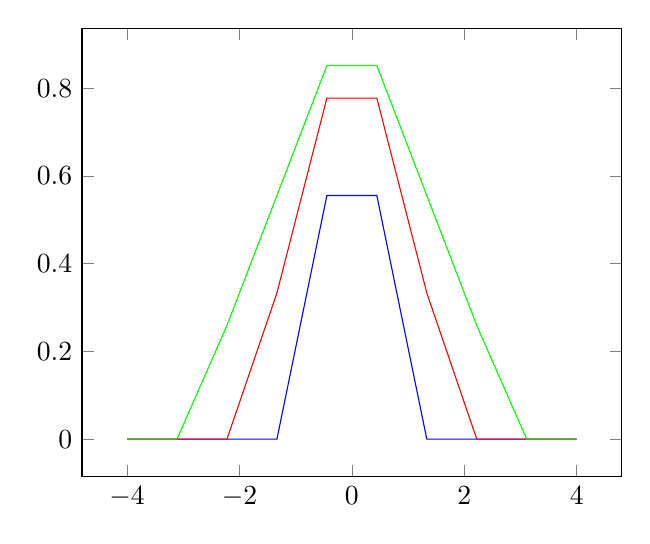
\begin{tikzpicture}
    \begin{axis}
    \addplot[domain=-4:4, samples=10, color=blue,]{max(x-1,0) + max(x+1,0) - 2*max(x,0)};
    \addplot[domain=-4:4, samples=10, color=red,]{max(x/2-1,0) + max(x/2+1,0) - 2*max(x/2,0)};
    \addplot[domain=-4:4, samples=10, color=green,]{max(x/3-1,0) + max(x/3+1,0) - 2*max(x/3,0)};
    \end{axis}
\end{tikzpicture}
    \caption{Illustration of the so-called ``bump'' function $\psi_a(x)$ used in the proof of \cref{lem:encoding-indicator-func2}. Here the colors of the displayed functions correspond to the parameter $a$ set to
    $a:=1$ in blue, $a:=2$ in red and $a:=3$ in green.}
    \label{fig:bump_function}
\end{figure}

\subsection*{Proofs}

\begin{proof}[\cref{lem:composition_lemma}]
    Let $\cC$ be a collection of functions computed by $\wlnn$, $h_1, \dots ,h_n \in \cC$, and $\mlp^\bullet$ a multilayer perceptron. Further, let $f_{1}, \ldots, f_{n}$ be the encoding functions, as well as $\text{MLP}_1, \ldots, \text{MLP}_n$ be the multilayer perceptrons used by $h_1, \dots h_n$ respectively. As outlined above, we will now construct $f^*$ and $\mlp^*$, such that for all graphs $G \in \xnn$:
    \begin{equation*}
        \mlp^\bullet(h_1(G), \dots ,h_n(G)) = \mlp^* \circ f^* \circ \wl(G)
    \end{equation*}
    such that we can conclude that the composition of multiple functions computable by $\wlnn$, is in fact also $\wlnn$ computable. 

    We define the new encoding function $f^*$ to work as follows on input $C_\infty$:
    \begin{equation*}
        f^*(C_\infty) := \textsf{concat}(
            \begin{bmatrix}
                f_1(C_\infty)\\
                \vdots\\
                f_n(C_\infty)
            \end{bmatrix}),
    \end{equation*}
    where $\textsf{conccat}$ is the concatenation functions, concatenating all encoding vectors to one single vector.

    Using the decomposition introduced in \cref{def:mlp}, we can decompose each $\mlp_i$ at layer $j > 1$ as follows: $(\mlp_i)_{j}(v) := \sigma(W^{i}_{j} \cdot (\mlp_i)_{j-1}(v) + b^i_j)$. Using this notation we construct $\mlp^*$ as follows:
    \begin{align*}
        &(\mlp^*)_{1}(v) := v\\
        &(\mlp^*)_{j+1}(v) := \sigma(W^*_j \cdot (\mlp^*)_{j} (v) + \textsf{concact}(
            \begin{bmatrix}
                b^1_j\\
                \vdots\\
                b^n_j
            \end{bmatrix})) &,\forall j \in [k]\\
        &(\mlp^*)_{j+k+1}(v) := (\mlp^\bullet)_{j+1}(v) &,\forall j \in [k^\bullet - 1]
    \end{align*}
    where $k$ is the maximum number of layers of the set of $\mlp_i$'s, $k^\bullet$ is the number of layers of the given $\mlp^\bullet$ and $\sigma$ an element wise activation function. Thereby, we define in the first equation line, that the start of the sequence is the input, with the second line, we construct the ``simultaneous'' execution of the $\mlp_i$'s, and in the last equation line, we add the layers of the given $\mlp^\bullet$ to the end. Further, we define the weight matrix $W_j^*$ as follows: 
    \begin{align*}
        W^*_j &:= \begin{bmatrix}
            W^1_j & 0 & \hdots & 0\\
            0 & W^2_j & \ddots & \vdots\\
            \vdots & \ddots & \ddots & 0\\
            0 & \hdots & 0 & W^n_j
        \end{bmatrix},
    \end{align*}
    such that we build a new matrix where each individual weight matrix is placed along the diagonal. Here we denote with $0$, zero matrices with the correct dimensions, such that $W_j^*$ is well-defined. Important to note, should for an $\mlp_i$, $W^i_j$ not exist, because it has less than $j$ layers, we use for $W^i_j$ the identity matrix $I_m$ where $m$ is the dimension of the output computed by $\mlp_i$.
\end{proof}





\setcitestyle{numbers}
\bibliography{references}
\end{document}